\chapter{Design and Implementation}
\label{chap3}
\section{Basic File Structure}

The \emph{/usr/src/servers/mfs} directory contains the source code for FS in
minx3.2 operating system. Some of the important files in mfs are \emph{main.c, inode.h, open.c, write.c, buf.h, super.h,
super.c,} etc. The main function of each file in \emph{mfs} are listed below:

% \begin{figure}[!htb]
%     \centering
%     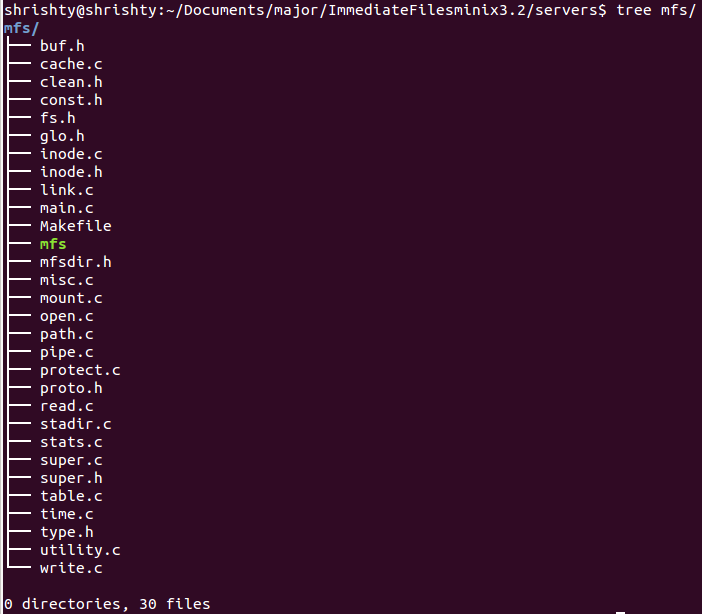
\includegraphics[scale=0.3]{img/minix_mfs_tree.png}
%     \caption{Main File System Structure}
% \end{figure}



\begin{itemize} 
\item \emph{buf.h} - Defines the block cache. It contains a \emph{union} named
\emph{fsdata\_u} with following attributes:
     \begin{itemize} 
        \item \emph{b\_\_data[MAX\_BLOCK\_SIZE]}, a character array, containing
        ordinary user data.
        \item
        \emph{b\_\_dir[NR\_DIR\_ENTRIES(\_MAX\_BLOCK\_SIZE)]} - directory block
        \item \emph{b\_\_bitmap[[FS\_BITMAP\_CHUNKS(\_MAX\_BLOCK\_SIZE)]]}
	  	- bitmap block
	  	\item direct and indirect inode blocks
     \end{itemize}
\item \emph{cache.c} - FS has a buffer cache to reduce the number of disk
accesses. File contains 9 procedures, few of them are listed below. 
	\begin{itemize} 
        \item \emph{get\_block} - Fetch a block for reading/writing. 
        \item \emph{put\_block} - Return a block
        \item \emph{rw\_block} - Transfer block between disk and cache
	  	\item \emph{free\_zone} - If file is deleted, free the zone
	  	\item \dots{}
     \end{itemize}
\item \emph{const.h} - Defines constants, like flags, table size that will be
used in the file system. Few constants are, \emph{IN\_CLEAN, IN\_DIRTY, ATIME,
CTIME} etc
\item \emph{fs.h} - Master header for FS, includes all header files needed by
the MFS source files.
\item \emph{glo.h} - Defines all the global variables. Few examples of global
variables are \emph{fs\_m\_in, fs\_m\_out, err\_code, fs\_dev,
user\_path[PATH\_MAX]} etc.
\item \emph{inode.h} - Contains the stucucture for \textit{inode} and the
\textit{inode\_table} as \emph{inode[NR\_INODES]}
\item \emph{inode.c} - Contains functions which manages the inode table. The
functions are \emph{get\_inode(), put\_inode(), rw\_inode(), alloc\_inode()} etc
\item \emph{main.c} - Contains the main routiene of the file system. The main
loop does three activities
	\begin{itemize} 
        \item \emph{get\_work(\&fs\_m\_in)} - Gets a new work 
        \item \emph{Processes} the work i.e. selects the fuction to be called
        to complete the work and calls it from the table of function pointers. 
        \item \emph{reply(src, \&fs\_m\_out)} - Sends a reply
     \end{itemize}
\item \emph{open.c} - Contains the codes for six system calls:\emph{open, close,
mknode, mkdir, close, lseek}
\item \emph{proto.h} - Lists all function prototypes for all functions used in
MFS
\item \emph{read.c} - All functions that are used for reading or writing are
present in read.c. Some of the functions include, \emph{fs\_readwrite,
rw\_chunk, read\_map} etc.
\item \emph{super.h} - Contains the superblock table. Super block holds
information about inode bitmap, zone bitmaps, inodes etc.
\item \emph{super.c} - Handles the superblock table and other related data
structures like zone bitmap, inode bitmap etc. Major functions in this file are:
\emph{alloc\_bit(), free\_bit(), get\_super(), read\_super()} etc.
\item \emph{table.c} - Contains the table that map system call numbers
onto the routines. 
\item \emph{write.c} - Contains files that are not in read.c but are necessary
for writing in a file. Most important functions in \emph{write.c} are
\emph{write\_map, clear\_zone, new\_block} and \emph{zero\_block}
 
\end{itemize}

\newpage
\section{Design and Algorithm Immediate File System}
There are two ways in which immediate files can be implemented in the
minix operating system:
\begin{itemize}

\item \emph{Static} - In this approach, the maximum file size is specified at
the creation time i.e. user himself specifies whether the file will be immediate
or regular and the file type cant be changed once it has been created. 
In case the immediate file size exceeds the specified size, it will report an error.
\item \emph{Dynamic} - A file is created as an immediate file and if size
exceeds specified size (of immediate files), it becomes a regular file. The user
doesn’t have to bother about the size of the file
\end{itemize}
We have used \emph{dynamic} approach in our project.

\subsection{Detailed Algorithm to include Immediate files}
\begin{algorithm}
\caption{Algorithm to include immediate files in the file system}
\label{IFSAlcorithm}
\begin{algorithmic}[1]
\Procedure{fs\_readwrite\_immed}{}
\State $is\_immediate$ = 0 (0 if regular, 1 if immediate)
\State $mode$ = inode.i\_mode ($regualar$ or $immediate$) 
\State $pos$ = req\_msg.LSEEK\_POS (lseek position)
\State $nrbytes$ = req\_msg.NBYTES (number if bytes to be read or written)
\State $rw\_flag$ = req\_msg.m\_type (READING or WRITING)
\State $f\_size$ = inode.f\_size
\State $immed\_buff[]$ = ``'' (temporary array)
\If{$mode$ == I\_IMMEDIATE}
\If{$rw\_flag$ == WRITING}
\If{($f\_size$ + nrbytes) \textgreater MAX\_IMMEDSIZE}
\If{($pos$ + $nrbytes$) \textless MAX\_IMMEDSIZE}
\State $i\_immediate$ = 1
\Else 
\State /** Shift from Immediate  to regular **/
\State Copy the content of zone to $immed\_buff$ array
\State Mark all zones as $empty\_zone$
\State Change $inode.size$ to zero
\State Change $update\_time$ of inode
\State Mark the inode $dirty$
\State Request a new block, $bp$
\State Copy the $immed\_buff$ content to $bp.data$ field
\State Mark the block, $bp$ dirty
\State Update $pos$ and $f\_size$
\State $inode.i\_mode$ = REGULAR
\State $is\_immediate$ = 0 // file is no more immediate
\EndIf
\Else 
\State $is\_immediate$ = 1
\EndIf
\Else 
\State /** reading no change required **/
\State $is\_immediate$ = 1
\EndIf
\EndIf
\If{$is\_immediate$ == 1} // the file is still immediate
\State Calculate the $zone\_position$ in the disk
\State Call $system\_read$ or $system\_write$ function with $zone\_pos$ as
argument
\EndIf
\EndProcedure
\end{algorithmic}
\end{algorithm} 

\newpage

\subsection{Implementation using dynamic approach}
This section will give an overview of what our algorithm actually does.

\subsubsection{Data Structures Involved}
All data strucutres which are related to our project are listed below
\begin{itemize}
  \item \emph{inode} - Structure of an inode in a disk is given in Figure2.2
  \begin{figure}[!htb]
    \centering
    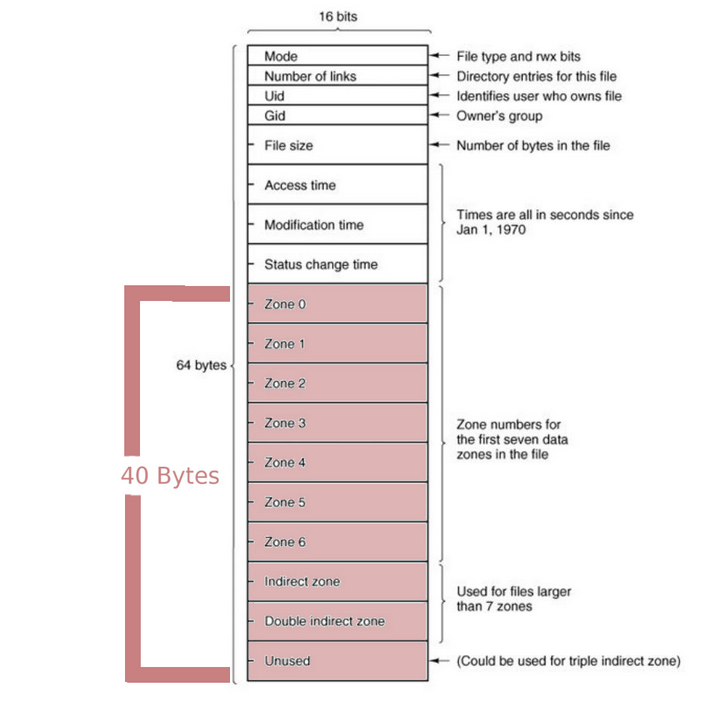
\includegraphics[scale=0.6]{img/inode.png}
    \caption{Inode Structure}
\end{figure} 


In Figure 2.2. we can see that there are 7 zones of 4 bytes each, an indirect
zone of size 4 bytes, a double indirect node of size 4 bytes and an unused space
of 4 bytes. Each zone points to a disk block where actual data gets stored. According
to definition of immediate files we had to find a space in the inode where we
can store the immediate files. These zones are apt place to store the immediate
files because no data which is critical to the file is being affected. We
calcualted \emph{maximum size} of immediate files as \emph{40 bytes} by adding
up sizes of all zones, indirect zones and unused space.

\begin{equation}
\boldsymbol{max\_size = zn\_sz * 7 + ud\_sz + idt\_sz + ddt\_sz} 
\end{equation}
\begin{equation}
\boldsymbol{\Rightarrow max\_size = 4 * 7 + 4 + 4 + 4 = 40 bytes}
\end{equation}

\item \emph{buffer or block cache} - This is a union of different types of
blocks in the disk. Eg. normal data block, directory block, inode block, bitmap
block etc. The design of buffer or block cache is given below,

\begin{lstlisting}
union fsdata_u {
	/* ordinary user data */
	char b__data[_MAX_BLOCK_SIZE]; 
	/* directory block */
	struct direct b__dir[NR_DIR_ENTRIES(_MAX_BLOCK_SIZE)];
	/* V1 indirect block */
	zone1_t b__v1_ind[V1_INDIRECTS];
	/* V2 indirect block */
	zone_t b__v2_ind[V2_INDIRECTS(_MAX_BLOCK_SIZE)];
	/* V1 inode block */
	d1_inode b__v1_ino[V1_INODES_PER_BLOCK];
	/* V2 inode block */
	d2_inode b__v2_ino[V2_INODES_PER_BLOCK(_MAX_BLOCK_SIZE)];
	/* bit map block */
	bitchunk_t b__bitmap[FS_BITMAP_CHUNKS(_MAX_BLOCK_SIZE)];
};

\end{lstlisting}
\emph{b\_\_data} array is used to cache the data which is stored in the disk
block, all the modifications by the user are done here and then the data is
written back to the disk. \emph{b\_data(b)} is a macro which returns the pointer
to the first byte of \emph{b\_\_data} array.

\item message - message structure is defined as follows
\begin{lstlisting}
typedef struct {
  int m_source;        // message source 
  int m_type;          // message type
  union {
        mess_1 m_m1;
        mess_2 m_m2;
        mess_3 m_m3;
        mess_4 m_m4;
        mess_5 m_m5;
        mess_7 m_m7;
        mess_8 m_m8;
  } m_u;
} message;
\end{lstlisting} 

\emph{mess\_1, mess\_2, mess\_3, \ldots} are different message types. In MFS,
global variables, \emph{fs\_m\_in} and \emph{fs\_m\_out}, of type \emph{message}
are used to send and recieve messages from various servers like VFS. Following
system calls are used for message passing: \emph{echo}, \emph{notify},
\emph{sendrec}, \emph{receive}, \emph{send}.
\end{itemize}

\newpage
\subsubsection{Files involved}
List of all files in which codes are added or deleted.

\begin{itemize}
  \item \emph{/src/include/const.h} - A new flag \emph{I\_IMMEDIATE} is created
  to support immediate files.
  \item \emph{src/sys/lib/libsa/minixfs3.h} - A new flag \emph{I\_IMMEDIATE} is created
  to support immediate files.
  \item \emph{/src/servers/vfs/open.c} - When \emph{O\_CREATE} flag is set. Set
  the file mode as immediate instead of regular. It will have size zero.
  \begin{lstlisting}
  	/* In function common_open */
	if (oflags & O_CREAT) {
	// we have removed I_REGULAR mode
        omode = I_IMMEDIATE | (omode & ALLPERMS & fp->fp_umask);
	vp = new_node(&resolve, oflags, omode);
	r = err_code;
	if (r == OK) exist = FALSE;	/* file created */
	else if (r != EEXIST) {		/* other error */
		if (vp) unlock_vnode(vp);
		unlock_filp(filp);
		return(r);
	}
  \end{lstlisting}
\item \emph{src/sys/sys/stat.h} - Following additions are done in this file:
	\begin{itemize}
	  \item \emph{\_S\_IFIMMED} - macro was defined, similar to regular files
	  \begin{lstlisting}
	  #define _S_IFIMMED 0130000      /* Immediate files */	
  	  \end{lstlisting}
  	  \item \emph{S\_IFIMMED} - macro redifined for easier usage, similar to
  	  regular files.
  	  \begin{lstlisting}
	  #define S_IFIMMED _S_IFIMMED    /* Immediate files */	
  	  \end{lstlisting}
  	  \item \emph{S\_ISIMMED(m)} - macro defined which checks whether a files is
  	  immediate or not (similar to regular files)
  	  \begin{lstlisting}
  	  /* Immediate */
	  #define S_ISIMMED(m) (((m) & _S_IFMT) == _S_IFIMMED) 	
  	  \end{lstlisting}
	\end{itemize}
\item There are \emph{114} more files where we have located \emph{S\_ISREG(m)}
and added \emph{S\_ISIMMED(m)} also in the code, because regular files and
immediate files have same functionalities except that immediate files are
stored in inode and regular files are stored in disk blocks pointed by zones in
the inode. Few of the files are listed below:
	\begin{itemize}
	  \item \emph{/servers/vfs/select.c}
	  \item \emph{/servers/vfs/link.c}
	  \item \emph{/servers/vfs/read.c}
	  \item \emph{/commands/grep/mmfile.c} \ldots etc
	\end{itemize}
\item \emph{/src/severs/mfs/read.c} - Major changes/addition for implementation
of immediate file system is done in this file, in the \emph{fs\_readwrite()}
function.
\begin{lstlisting}
/** in File read.c **/
/** start **/
cum_io = 0;
char immed_buff[41];
if ((rip->i_mode & I_TYPE) == I_IMMEDIATE) {
	int is_immediate;
	int i;
	if (rw_flag == WRITING) {
	 if ((f_size + nrbytes) > 40) {
	   if (position == 0 && nrbytes <= 40) {
		  is_immediate = 1;
		} else {
		  register struct buf *bp;
		  for (i = 0; i < f_size; i++) {
		    immed_buff[i] = *(((char *) rip->i_zone)+i);
		  }

		  for (i = 0; i < V2_NR_TZONES; i++) {
		    rip->i_zone[i] = NO_ZONE;
		  }
		  rip->i_size = 0;
		  rip->i_update = ATIME | CTIME | MTIME;
		  IN_MARKDIRTY(rip);

		  bp = new_block(rip, (off_t) 0);

		  if (bp == NULL)
		    panic("error");

		  for (i = 0; i < f_size; i++) {
		    b_data(bp)[i] = immed_buff[i];
		  }

		  MARKDIRTY(bp);
		  put_block(bp, PARTIAL_DATA_BLOCK);

		  // same as after rw_chunk is called
		  position += f_size;
		  f_size = rip->i_size;
		  rip->i_mode = I_REGULAR;
		  is_immediate = 0;
		}
	 } else {
		 is_immediate = 1;
	 }
 }
	if (is_immediate == 1) {
		if (rw_flag == READING) {
			r = sys_safecopyto(VFS_PROC_NR, gid, 
			(vir_bytes) cum_io, 
			(vir_bytes)(rip->i_zone + position), 
			(size_t) nrbytes);
		} else {
			r = sys_safecopyfrom(VFS_PROC_NR, gid, 
			(vir_bytes) cum_io,
			(vir_bytes)(rip->i_zone + position), 
			(size_t) nrbytes);
			IN_MARKDIRTY(rip);
		}

		if (r == OK) {
			cum_io += nrbytes;
			position += nrbytes;
			nrbytes = 0;
		}
		for (int i = 0; i < f_size; i++) {
			immed_buff[i] = *(((char *) rip->i_zone)+i);
		}
		printf("immedbuf: %s\n", immed_buff);
	}
}
/** end **/
	  	
\end{lstlisting}   
\end{itemize} 
 




